\documentclass{article}
\usepackage{amsmath}
\usepackage{amssymb}
\usepackage{amsthm}
\usepackage[utf8]{inputenc}
\usepackage{amsmath}
\usepackage{amsfonts}
\usepackage[]{graphicx}
\usepackage[a4paper, portrait, margin = 1in]{geometry}
\usepackage{enumitem}
\usepackage{xcolor}

%darkmode
%\pagecolor[rgb]{0.2,0.19,0.18} 
%\color[rgb]{0.92,0.86,0.7}

\newenvironment*{alphenum}{\begin{enumerate}[label= (\alph*)]}{\end{enumerate}}

\pagestyle{fancy}
\lhead{Assignment \# $3$}
\rhead{Name: Thomas Boyko; UCID: 30191728}
\chead{}

\begin{document}
\begin{enumerate} 
\item Consider the function $f:\mathbb{R}^3\to\mathbb{R}^3$, defined by  
$f(x,y,z)=\begin{pmatrix}
x^3-y-z\\2x+y+z\\x+y-z
\end{pmatrix}$  
\begin{enumerate}[label= (\alph*)] 
    \item Compute $Jf(x,y,z)$ and show that $\mathrm{d}f_{(x,y,z)}$ is invertible for any $(x,y,z)\in\mathbb{R}^3$.  
    \paragraph{Solution: } Compute:
    \[
     Jf(x,y,z)=\begin{bmatrix}\frac{\partial f_1}{\partial x}&\frac{\partial f_1}{\partial y}&\frac{\partial f_1}{\partial z}\\\frac{\partial f_2}{\partial x}&\frac{\partial f_2}{\partial y}&\frac{\partial f_2}{\partial z}\\ \frac{\partial f_3}{\partial x}&\frac{\partial f_3}{\partial y}&\frac{\partial f_3}{\partial z}\end{bmatrix}
     =\begin{bmatrix} 3x^2&-1&-1\\
     2&1&1\\
     1&1&-1 \end{bmatrix} 
    .\] 
    Then we take the determinant;
    \[
        \det Jf(x,y,z)=3x^2\begin{vmatrix} 1&1\\1&-1 \end{vmatrix} -2\begin{vmatrix} -1&-1\\1&-1 \end{vmatrix} +\begin{vmatrix} -1&-1\\1&1 \end{vmatrix} =-6x^2-4+0
    .\] 
    And we can see that since this determinant has no real roots, it must be nonzero for any $(x,y,z)\in \mathbb{R}^3$, and so $Jf$, as well as $df$ are both invertible in $\mathbb{R}^3$.

    \item Find the largest open $U\subset\mathbb{R}^3$ where $f$ has a continuously differentiable inverse function $g.$  
        \paragraph{Solution: }Begin by showing that $f$ is injective in $\mathbb{R}^3$. Suppose:
        \begin{align*}
            x_1^3-y_1-z_1&=x_2^3-y_2-z_2\tag{1}\\
            2x_1+y_1+z_1&=2x_2+y_2+z_2\tag{2}\\
            x_1+y_1-z_1&=x_2+y_2-z_2\tag{3}
        .\end{align*}
        However, if we add $(1)+(2)$, we get $x_1^3+2x_1=x_1(x_1^2+2)=x_2(x_2^2+2)=x_2^3+2x_2$.
        Let $h(x)=x^3+2x$, so that $h'(x)=3x^2+2$, positive for all $x$. So then $h$ is increasing, and therefore injective, and since  $h(x_1)=h(x_2),$ we must have $x_1=x_2$. Then we can transform $(2),(3):$ 
         \begin{align*}
            y_1+z_1-y_2-z_2&= 0 \\
            y_1-z_1-y_2+z_2&= 0 
        .\end{align*}
        And we transform this homogenous system into a matrix to put into RREF:
        \begin{align*}
            \begin{bmatrix}1&1&-1&-1\\
                1&-1&-1&1\end{bmatrix}\begin{bmatrix} y_1\\z_1\\y_2\\z_2\end{bmatrix}=0\\
                \begin{bmatrix}1&0&-1&0\\
                0&1&0&-1\end{bmatrix}
                \begin{bmatrix} y_1\\z_1\\y_2\\z_2\end{bmatrix}=0\\
        .\end{align*}
        And so we have $x_1=x_2,y_1=y_2,z_1=z_2$ as desired, and $f$ is injective in $\mathbb{R}^3$, and clearly $f(\mathbb{R}^3)=\mathbb{R}^3$.

        Then since $f$ is injective in $\mathbb{R}^3$ and $df$ is invertible in $\mathbb{R}^3$, by the Global inversion theorem, $U=\mathbb{R}^3$ is the largest open set in which $f$ is invertible.

\end{enumerate}
\newpage

\item Consider the system of equations:
$(S) \left\{\begin{array}{l}
x - y - u^2 + v^2 = 0 \\
x + y - 2uv = 0
\end{array}\right.$  
\begin{enumerate}[label= (\alph*)] 
    \item Show that the system $(S)$ can be solved for $u,v$ in term of $(x,y)$ near the point $(x,y,u,v)=(1,1,1,1).$  
        \paragraph{Solution: }We solve for the Jacobian about $(1,1,1,1)$.
         \[ Jf(x,y,u,v)=\begin{bmatrix} 
        1&-1&-2u&2v\\
        1&1&-2v&-2u \end{bmatrix} \]
        \[
        Jf(1,1,1,1)=\begin{bmatrix} 
        1&-1&-2&2\\
        1&1&-2&-2 \end{bmatrix}
        .\] 
        And if we break $Jf$ into block matrices, we get the right half of $Jf$, $\partial_{u,v}f=\begin{bmatrix} -2&2\\-2&-2 \end{bmatrix} $ which has nonzero determinant and must be invertible. So $u,v$ can be implicitly defined about $(1,1,1,1)$ by the Implicit Function theorem. 
    \item Compute $\partial_x u(1,1)+\partial_y v(1,1)$.

        \paragraph{Solution: }Begin with the identity from the Implicit Function Theorem:
        \begin{align*}
            \begin{bmatrix}  \partial_x u&\partial_y u\\\partial_x v&\partial_y v\end{bmatrix} 
            &= \begin{bmatrix}  \partial_u f_1&\partial_v f_1\\\partial_u f_2&\partial_v f_2\end{bmatrix}^{-1}
            \begin{bmatrix}  \partial_x f_1&\partial_y f_1\\\partial_x f_2&\partial_y f_2\end{bmatrix}\\
               &=\left(\det\begin{bmatrix} -2u&2v\\-2v&-2u\end{bmatrix}\right)^{-1}  \begin{bmatrix} -2u&-2v\\2v&-2u\end{bmatrix}
            \begin{bmatrix} 1&-1\\1&1 \end{bmatrix} \\
            &= \frac{1}{2(u^2+v^2)} \begin{bmatrix} -u&-v\\v&-u\end{bmatrix}
            \begin{bmatrix} 1&-1\\1&1 \end{bmatrix} \\
                 &= \frac{1}{2(u^2+v^2)} \begin{bmatrix} -u-v&u-v\\v-u&-v-u \end{bmatrix}
        .\end{align*}
        And so if we want the sum $\partial_x u(1,1)+\partial_y v(1,1)$ we need only take the trace of this matrix and evaluate at $(1,1)$.
        \begin{align*}
             \partial_x u(1,1)+\partial_y v(1,1)&= \frac{1}{2(u^2+v^2)} \bigg|_{(1,1)}\\
             &= -2\frac{u+v}{2(u^2+v^2)} \bigg|_{(1,1)}\\
             &= -1 
        .\end{align*}
\end{enumerate}

\item   Let $f:\mathbb{R}^2\to\mathbb{R}:(x,y)\to f(x,y).$ Show that if $f\in C^1(\mathbb{R}^2,\mathbb{R}),$ then $f$ can't be injective on $\mathbb{R}^2.$ Hint: Use the implicit functions theorem.
    \paragraph{Solution: } Assume, for the purpose of deriving a contradiction, that $f$ is injective on $\mathbb{R}^2$. Let $(a,b)\in \mathbb{R}^2$, and note that $c=f(a,b)$ is only attained at $(a,b)$. Take the derivative; 
    \[
        df=[\partial_x f\quad \partial_y f]
    .\] 
    If $\partial_yf(a,b)\neq 0$, there exists some function $g:\mathbb{R}\to \mathbb{R}$, so that $c=f(x,g(x))$, for all $(x,y)$ close to $(a,b)$ within a neighborhood $U$ of $(a,b)$. But then we have multiple distinct points mapping to $p$, and then $\partial_Yf(a,b)=0$.

    Otherwise, if $\partial_yf=0$, we check $\partial_xf$. If this is nonzero, we repeat the above argument with ImFT for $x$, to get $\partial_xf(a,b)=0$.

    Since $(a,b)$ was chosen arbitrarily, we must have $df=0$ for any $(x,y)\in \mathbb{R}^2$. The only functions for which this holds true are constant, and since constant functions are not injective, $f$ cannot be injective.

    \newpage
\item  Let $E=C([a,b],\mathbb{R})$ equipped with the norm of uniform convergence, let $u\in C(\mathbb{R},\mathbb{R}),$ and consider the mapping $\phi:E\to E,$ defined by $\phi(v)=u\circ v.$ Is $\phi$ continuous? Make sure to justify your answer.
    \paragraph{Solution: } Let $\varepsilon>0$, and $v,w\in E$. Recall that the image of compact sets under continuous functions is compact, and the union of compact sets is compact. Then since continuous functions are uniformly continuous on compact sets, $u$ must be uniformly continuous on $v([a,b])\cup w([a,b])$. Let $x\in [a,b]$, and let $\delta$ be chosen so that $|w(x)-v(x)|<\delta\implies|u(w(x))-u(v(x))|<\varepsilon$. 
    Suppose
    \[
        \|w-v\|= \sup_{x\in [a,b]}|w(x)-v(x)| <\delta \tag{$*$}
    .\] 
    Then we must have $|w(x)-v(x)|<\delta$ for any $x\in [a,b]$. But by continuity of $u$, we have 
    \[ |\phi(w)-\phi(v)|=|u(w(x))-u(v(x))|<\varepsilon .\] 
    for any $x\in [a,b]$. Then recall that since $u,v,w\in E$ are continuous, the composition, difference and absolute value $|u\circ w-u\circ v|$ is continuous. Therefore the supremum of this function is attained in the compact set $[a,b]$, and when we take the supremum $\sup_{x\in [a,b]}|u(w(x))-u(v(x))|$, we can say that it is attained for some $x_0\in [a,b]$. And from ($*$), we have:
    \begin{align*}
        \|\phi(w)-\phi(v)\|&=\|u\circ w-u\circ v\|\\
                           &=\sup_{x\in [a,b]}|u(w(x))-u(v(x))|\\
                           &=|u(w(x_0))-u(v(x_0))|\\
                           &<\varepsilon
    .\end{align*}
    And $\phi$ is continuous as desired.

\item  Find in $C([0,1],\mathbb{R})$ the distance from the function $u(t)=t$ to the subspace $\mathbb{P}_0$ of polynomials of degree $0.$ Make sure to justify your answer.
    \paragraph{Solution: }Let $u(t)=t$, and take the distance:
    \begin{align*}
        d(u,\mathbb{P}_0)&=\inf_{p\in \mathbb{P}_0}d(u,p)\\
        &= \inf_{c\in \mathbb{R}}\|u-c\| &\text{$p$ is simply a real constant}\\
        &= \inf_{c\in \mathbb{R}}\sup_{t\in [0,1]}|u(t)-c|\\
        &= \inf_{c\in \mathbb{R}}\sup_{t\in [0,1]}|t-c|
    .\end{align*}

    Write $f_c(t)=|t-c|$. This continuous function will attain its supremum in the compact $[0,1]$. Since $|t-c|$ is decreasing on $(-\infty,c]$ and increasing on $[c,\infty)$, the supremum must be either at $0$ or $1$. So we can rewrite $d(u,\mathbb{P})=\inf_{c\in \mathbb{R}}\max \{|c|,|1-c|\} $.

    We claim that $\frac{1}{2}$ is this infimum. First we show that this is a lower bound; let $c\in \mathbb{R}$. If $c<\frac{1}{2}$, then $|c|<\frac{1}{2}, |1-c|>\frac{1}{2}$, and so $\frac{1}{2}<\max \{|c|,|1-c|\}=|1-c|$. 

    Now if $c>\frac{1}{2},$ we have $|1-c|<\frac{1}{2}$, $|c|>\frac{1}{2}$ and so $\frac{1}{2}<\max \{|c|,|1-c|\}=|c|$. 

    Finally, if $c=\frac{1}{2}$, we have $\max \left\{ |\frac{1}{2}|,|1-\frac{1}{2}| \right\} =\frac{1}{2}$. All this is to say that $\frac{1}{2}$ is the greatest lower bound for this set of maximums, and therefore $d(u,\mathbb{P}_0)=\frac{1}{2}$

    \iffalse 
        \begin{tikzpicture}
        \tzaxes(-1,-1)(3,3){$t$}{}
        \tzfn[thick]{abs(\x-1.5)}[-1:3]{}[al]
        \tzfn[thick]{abs(\x+.5)}[-1:3]{}[al]
        \tzfn[thick]{abs(\x-.5)}[-1:3]{}[al]
        \tzvfnat[dotted,thick]{1}[0:3]
        \end{tikzpicture}
    \fi

\newpage

\item  Let $f\in C([a,b],\mathbb{R})$ be such that $\int_a^b f(x)x^n\operatorname{dx}=0,\quad\forall n\in\mathbb{N}$ Show that $f$ is identically zero. Hint: Use Weierstrass Theorem.
    \paragraph{Solution: }First, we claim that if $p$ is any real polynomial, then $\int_{a}^{b} f(x)p(x) \, d x =0$. Write $p=\sum_{i=0}^{n} c_ix^{i}$. Then:
    \begin{align*}
    \int_{a}^{b} f(x)p(x) \, d x &=\int_{a}^{b} f(x)\sum_{i=0}^{n} c_ix^{i} \, d x \\&=\sum_{i=0}^{n} \int_{a}^{b} c_ix^{i}f(x) \, d x \\&=\sum_{i=0}^{n}c_i \int_{a}^{b} x^{i}f(x) \, d x \\&=\sum_{i=1}^{n} c_i \cdot 0\\&=0
    .\end{align*}
    By Weierstrass, there exists a sequence of real polynomials convergent to $f$. Let $\{p_n\}$ be such a sequence, and take:
    \begin{align*}
        \int_{a}^{b} f^2(x) \, d x &= \int_{a}^{b} \lim_{n \to \infty} p_n(x) f(x)\, d x  \\
           &= \lim_{n \to \infty} \int_{a}^{b} f(x)p_n(x) \, d x  &\text{$fp_n\in C([a,b])$ }\\
        &= \lim_{n \to \infty} 0 \\
        &= 0 
    .\end{align*}
    Define $F(x)$ so that $\frac{d}{dx}F(x)=f^2(x)$ by the Fundamental Theorem of Calculus. Then $\int_{a}^{b} f^2(x) \, d x =F(a)-F(b)=0$. Then $F(a)=F(b)$. But since $f^2(x)\ge 0$, $F$ is increasing, and we must have $F(x)=c$ for some constant real $c\in \mathbb{R}$. Then since $f^2(x)=\frac{d}{dx}F(x)=\frac{d}{dx}c=0$, we have $f^2$ is identically $0$, and then $f$ must also be identically $0$.
\end{enumerate}
\end{document}
